\section{Simple Machines}

%Levers


%Pulleys


\subsection{Pulley}

\subsubsection*{Learning Objectives}
\begin{itemize}
\item{To determine the mechanical advantage, velocity ratio and efficiency of a pulley system}
\end{itemize}

\subsubsection*{Background Information}
A pulley is a wheel which can be turned by a rope or string.  You can have many pulleys in different configurations in order to reduce the effort needed to do work.
The mechanical advantage of a pulley is calculated by dividing the load by the effort needed to lift the load.
$$\mathrm{mechanical \;advantage} = \frac{\mathrm{load}}{\mathrm{effort}}$$
The velocity ratio of a pulley is calculated by dividing the distance moved by the effort by the distance moved by the load.  This is also equal to the number of pulleys in the system.
The efficiency of the pulley and all other simple machines is equal to the mechanical advantage divided by the velocity ratio.

\subsubsection*{Materials}
Piece of cardboard from a box, thread, stones, spring balance (see the ``Spring Balance" activity in order to make one), two empty water bottles, retort stand or piece of wood

\subsubsection*{Preparation Procedure}
\begin{enumerate}
\item{Cut off the tops of the water bottles just below the lip where the cap rests.}
\item{Cut the piece of cardboard into two equal size pieces.  They should be at least 5 cm squares.}
\item{In the middle of each piece of cardboard, cut a hole just big enough for the water bottle tops to fit through.}
\item{Thread the water bottle tops into the holes so that they are secure.}
\item{Make a small hole near the edge of each piece of cardboard.}
\item{Fix one of the cardboard pieces vertically on a retort stand or up high on a piece of wood.}
\item{Tie a piece of thread to the hole in the cardboard on the retort stand.}
\item{Fix a stone or other weight to the other cardboard piece and measure its weight, or measure its mass and convert this to weight.}
\item{Use the thread to suspend one of the cardboard pieces from the piece on the retort stand.  Pass the thread over the rails of the water bottle tops so that it can roll over the thread like a pulley.  Extend the thread back up to the top of the retort stand and wrap it over the top of the water bottle top.}
\item{Place a metre rule on the retort stand.}
\item{Attach the free end of the thread to a spring balance which can be pulled down to lift the load on the pulley at the bottom.  You now have a pulley system consisting of one fixed pulley and one move-able pulley.}
\end{enumerate}

\begin{figure}
\begin{center}
%\def\svgwidth{150pt}
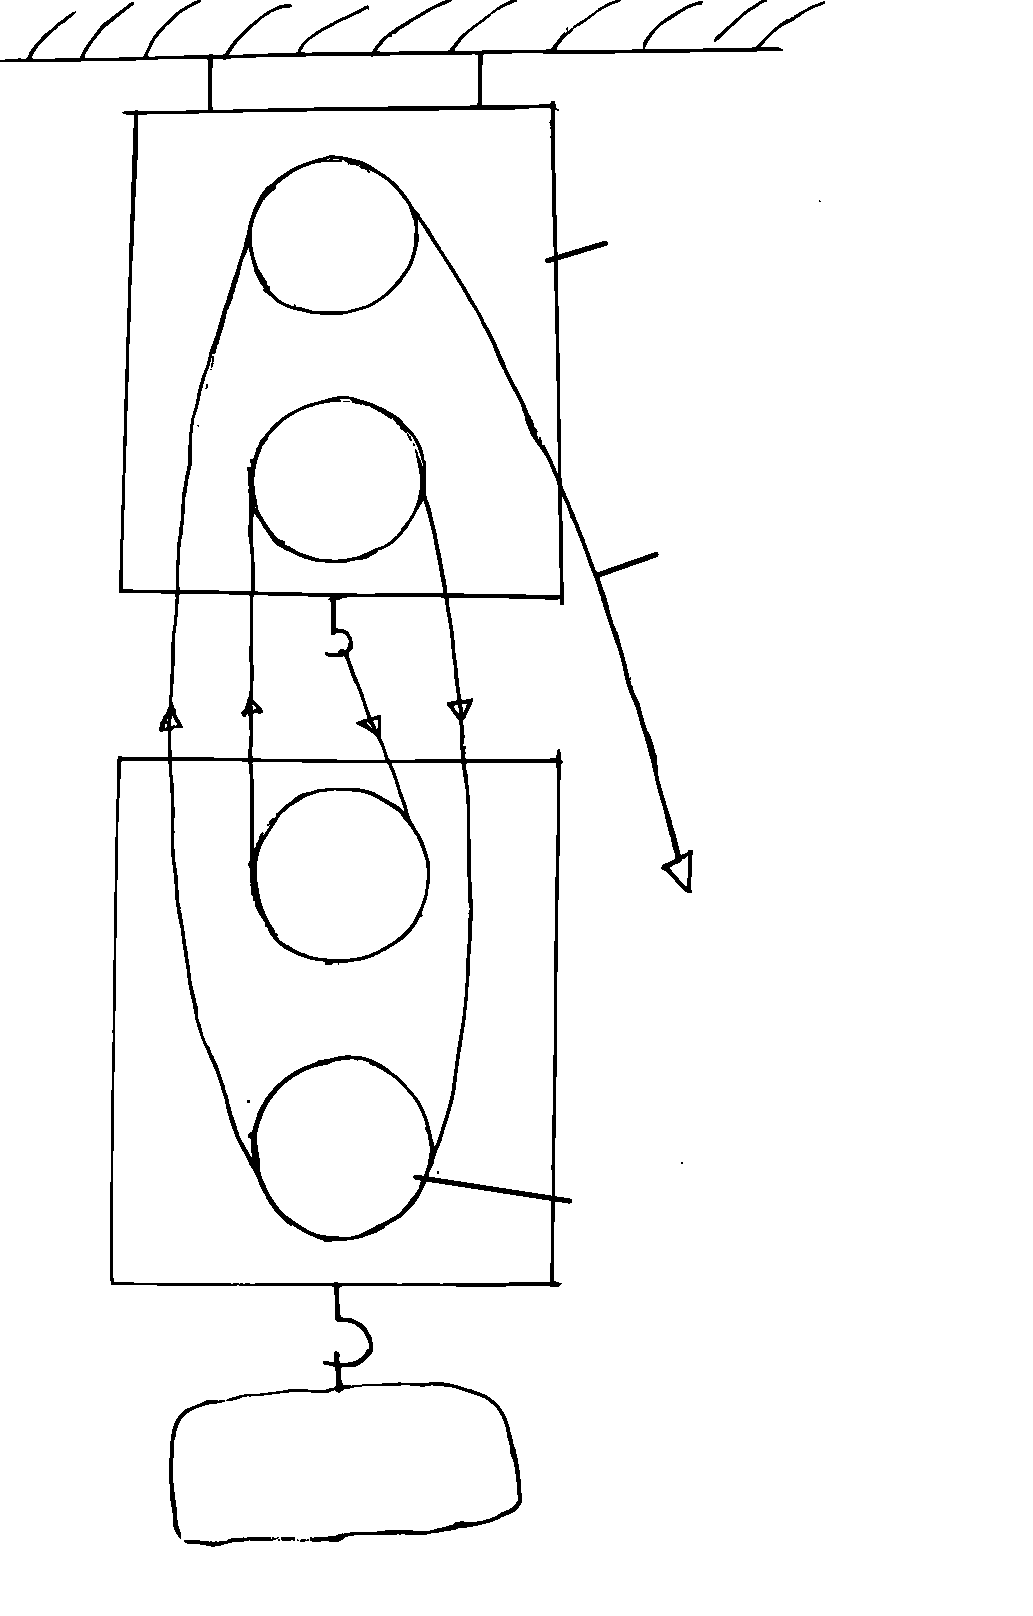
\includegraphics{./img/block-n-tackle.png}
\caption{Simple Machines: The Pulley}
\label{fig:block-n-tackle}
\end{center}
\end{figure}

\subsubsection*{Activity Procedure}
\begin{enumerate}
\item{Pull the spring balance down a certain distance and record the distance moved by the load (the lower pulley with the stone) and the effort (the spring balance).}
\item{Use these distances to calculate the velocity ratio of the pulley system.}
\item{Record the force used on the spring balance to life the load.}
\item{Use this force and the weight of the load to calculate the mechanical advantage of the pulley system.}
\item{Use your calculated values of velocity ratio and mechanical advantage to calculate the efficiency of the pulley system.}
\end{enumerate}

\subsubsection*{Results and Conclusions}
The velocity ratio calculated by measuring the lengths is equal to the number of pulleys in the system, in this case two.  When this number is divided from the mechanical advantage, the efficiency of the system should be close to 100\% (the ratio is 1).  It will not be exactly 100\% because there is friction in the system which reduces the mechanical advantage.


\subsubsection*{Discussion Questions}
\begin{enumerate}
\item{What is the relationship between the distance moved by the load and the distance moved by the effort for this pulley system?}
\item{Compare the velocity ratio of this system to the number of pulleys present.}
\item{What would be the velocity ratio of a pulley system with 5 pulleys?}
\item{What was the mechanical advantage of this system?}
\item{What was the efficiency for this system?}
\item{Why is the efficiency not exactly 100\%?}
\end{enumerate}

\subsubsection*{Notes}
The efficiency of this pulley will not be 100\% because of friction.  Try to use other resources to make a better pulley in order to reduce the effect of friction.



%Inclined Plane

\subsection{Pulleys and Inclined Planes}
\begin{itemize}
\item{Preparation Time: 15 minutes}
\item{Materials: thread spool or water bottle, cardboard, thread: meter rule, spring or spring balance, various masses, stiff wire}
\item{Procedure – Pulleys: A thread spool works well as a pulley, but you can also cut out the ridged section of a water bottle and insert a circle of cardboard into the center as a support. Bend the stiff wire through the hole of the pulley so it can rotate easily without sliding off. Tie the masses to the thread and drape it over the pulley. You can make any fixed or moveable pulley with these resources.}
\item{Procedure – Inclined Planes: Prop up a meter rule at an angle. Hang a mass from a spring or spring balance and drag it up the slope. Measure the extension of the spring (or weight) for the mass when it hangs freely, and again as it moves up the slope. If friction is low, there will be a noticeable decrease in spring extension from the free-hanging mass to the mass on the slope.}
\end{itemize}


%Screw and Screw Jack


%Wheel and Axle (gears)

\subsection{Bottle Cap Gearworks}
\begin{itemize}
\item{Preparation Time: 30 minutes}
\item{Materials: handful of bottle caps, pliers, nails, small piece of flat wood, hammer}
\item{Procedure: Find the exact center of each bottle cap and poke a hole through it for the nail. Bend the edges of the bottle caps in so that the ridges along the sides will act as gear teeth when the cap rotates. Nail the caps into the wood at even intervals so that they can freely rotate and in turn cause others to rotate. Make different configurations and note the direction of rotation from one gear to another.}
\end{itemize}


%Hydraulic Press

